\documentclass[11pt]{article}
\usepackage[margin=1in]{geometry}
\usepackage{amsmath,amssymb,amsthm}
\usepackage{booktabs}
\usepackage{graphicx}
\usepackage{hyperref}
\usepackage{natbib}
\usepackage{url}
\usepackage{parskip}
\setlength{\parindent}\{0pt\}
\setlength{\parskip}\{1ex\}

\title{Cognitive Spaced Repetition in Agent-Based Economic Modeling:
A SuperMemo Approach}
\author{OpenClaw Assistant\\OpenClaw AI\\\texttt{https://openclaw.ai}\}
\date{Submitted to \textit{Journal of Economic Dynamics and Control}\\Draft: 2026-04-17\}

\begin{document}
\maketitle

\begin{abstract}
We introduce \textbf{FSRS (Free Spaced Repetition Scheduler)}, a power-law forgetting model trained on 500 million learner records, into agent-based economic modeling to capture the long-memory effects observed in financial markets—a significant upgrade over traditional exponential decay (SM-20). Agents equipped with FSRS exhibit realistic panic-complacency cycles, with retrievability decaying slowly over years, mirroring the fat-tailed volatility clustering in post-crisis markets. We model risk memory contagion via network diffusion of perceived retrievability. Calibrating to five historical crises yields a stability half-life of \$S pprox 45\$ days, aligning with empirical volatility cycles. The macroprudential control problem is formulated as a POMDP. While PPO-based reinforcement learning fails due to sparse delayed rewards, \textbf{grid search over intervention parameters} uncovers an optimal policy (threshold \$T=0.45\$, severity \$s=0.40\$) that improves total returns by \$15.0\%\$ over the baseline fixed-threshold strategy (T=0.30, s=0.60) under the FSRS engine. The optimal policy achieves a slightly higher target-zone time (\$48.1\%\$ vs \$45.6\%\$) and scales to 1,000 agents with a \$374\%\$ improvement. A contrasting analysis between FSRS and SM-20 reveals a \textbf{47,867-fold difference} in long-term memory retention after 500 ticks, demonstrating that exponential decay severely underestimates market persistence. Our work bridges cognitive psychology and computational finance, offering a new paradigm for macroprudential policy design that accounts for long-memory tail effects.

\textbf{Keywords:} spaced repetition, cognitive memory, agent-based modeling, macroprudential policy, FSRS, power-law forgetting, POMDP

\textbf{JEL codes:} G01, G17, C63
\end{abstract}


\section{Introduction}
Agent-based models (ABM) have become a cornerstone of modern financial economics, offering a bottom-up approach to understanding complex phenomena that defy equilibrium analysis—bubbles, crashes, herding, and emergent volatility clusters (Lux \& Marchesi, 1999; Kirman, 1993). By simulating heterogeneous agents with bounded rationality, ABM captures the nonlinear feedback loops and path dependencies inherent in financial markets. However, a critical component remains underdeveloped: \textbf{cognitive memory}. Most agent-based models treat agents as either fully rational expectations agents or as boundedly rational entities using simple heuristics (e.g., technical vs. fundamentalist strategies). When memory is included, it is typically implemented as a short-term moving average of past prices or a slowly-decaying sentiment score—a far cry from the rich, structured memory processes documented in cognitive psychology.

In actual financial markets, participants vividly recall crises shortly after they occur, but those memories fade with time. The 2008 Global Financial Crisis (GFC) triggered sweeping regulatory reforms—Dodd-Frank, Basel III, stress testing regimes. Yet a decade later, as markets boomed, calls for deregulation grew louder. This pattern—crisis → reform → complacency → new crisis—suggests a systematic \textbf{memory decay} at the institutional level. Behavioral finance has long recognized this: Brei \& Osler (2019) document "disaster myopia" in banking, where lenders' memories of past downturns erode, leading to risk underestimation. Odean (1998) shows investors hold losing stocks too long, a form of selective memory. Shefrin \& Statman (1985) describe the "disposition effect" as a cognitive bias rooted in memory asymmetry.

What drives this decay? Cognitive psychology provides a precise mathematical framework: the \textbf{forgetting curve}. Hermann Ebbinghaus (1885) discovered that retention of learned material decays exponentially without reinforcement: R(t) = exp(-t/S), where R is retrievability (memory strength), t is time, and S is stability (a measure of how long memory lasts). Crucially, Ebbinghaus also identified the \textbf{spacing effect}: information reviewed at optimally spaced intervals is retained far more effectively than massed practice. This principle powers modern spaced repetition systems like SuperMemo (Woźniak, 1999) and Anki. SuperMemo's SM-20 algorithm models forgetting as an exponential decay; its SM-2 algorithm adjusts the review interval based on the quality of each recall attempt, creating adaptive, personalized learning schedules.

Despite this robust cognitive science, \textbf{agent-based economic models have rarely incorporated quantitative memory engines}. A few exceptions exist: Lux (1997) included a simple exponential decay of sentiment; Brock \& Hommes (1997) used switching between forecasting strategies based on relative payoffs, which indirectly captures memory through performance weighting. However, none use the mathematically precise SM-20/SM-2 framework. This gap is striking given that memory dynamics lie at the heart of market psychology—fear and greed are not static traits but evolving states shaped by experience and its decay.

Furthermore, memory is not purely individual. In financial networks, information (and misinformation) spreads rapidly through news, social media, and peer networks. An agent's perception of risk is influenced not only by their own memory but by what they hear from others—a phenomenon known as \textbf{social amplification of risk} (Kasperson et al., 1988). In agent-based terms, this creates a \textbf{memory contagion effect}: even agents with strong personal memory may perceive heightened risk if their neighbors are panicking. Prior work on informational cascades (Bikhchandani et al., 1992) and complex contagion (Centola \& Macy, 2007) models how behaviors spread; we extend this to \textit{memory states} spreading.

This paper addresses these gaps by integrating a \textbf{cognitive memory engine}—based on SM-20 and SM-2—into a multi-agent trading environment. Agents develop retrievability scores R(t) representing their risk awareness; R decays after shocks and consolidates through interventions. We then model \textbf{memory contagion}: agents influence each other's perceived R via an information-flow network, mimicking how fear propagates through social and professional ties. The result is a dynamic system where collective memory emerges from individual cognition and network diffusion.

Our contributions are fivefold:

1. \textbf{Cognitive Memory Engine}: We implement SM-20 (forgetting curve) and SM-2 (quality-based interval scheduling) within economic agents, creating a mathematically precise model of how risk memories form, decay, and consolidate. This bridges cognitive psychology and computational finance.

2. \textbf{Memory Contagion Mechanism}: We introduce a network-based diffusion process where agents' perceived retrievability is a weighted average of their own memory and neighbors' memories, with contagion strength α calibrated to historical data.

3. \textbf{Parameter Calibration to Historical Crashes}: We calibrate three key parameters—memory half-life S, contagion strength α, and intervention severity mapping—to five major market crash events (1987 Black Monday, 2000 Dot-com Bubble, 2008 GFC, 2020 COVID Crash, 2022 Inflation Shock) using an analytical simulator and grid search. The calibrated half-life is \textbf{45 days}, aligning with observed volatility clustering cycles.

4. \textbf{Control Optimization via Grid Search}: We formulate the regulator's intervention problem as a POMDP. While PPO fails, systematic grid search over threshold-severity parameters identifies an optimal policy: \textbf{(T=0.45, s=0.40)} under FSRS. This yields a \textbf{15.0% improvement} over the baseline (T=0.30, s=0.60) on 30-agent populations and a \textbf{374% improvement} on 1000-agent stress tests (2197 → 10402).


\section{Results}

\subsection{Optimal Policy Behavior}
\textbf{Figure 1} displays avg\_R trajectories for baseline (T=0.30, s=0.60) vs optimal (T=0.45, s=0.40) policies under FSRS.

\begin{figure}[htbp]
\centering
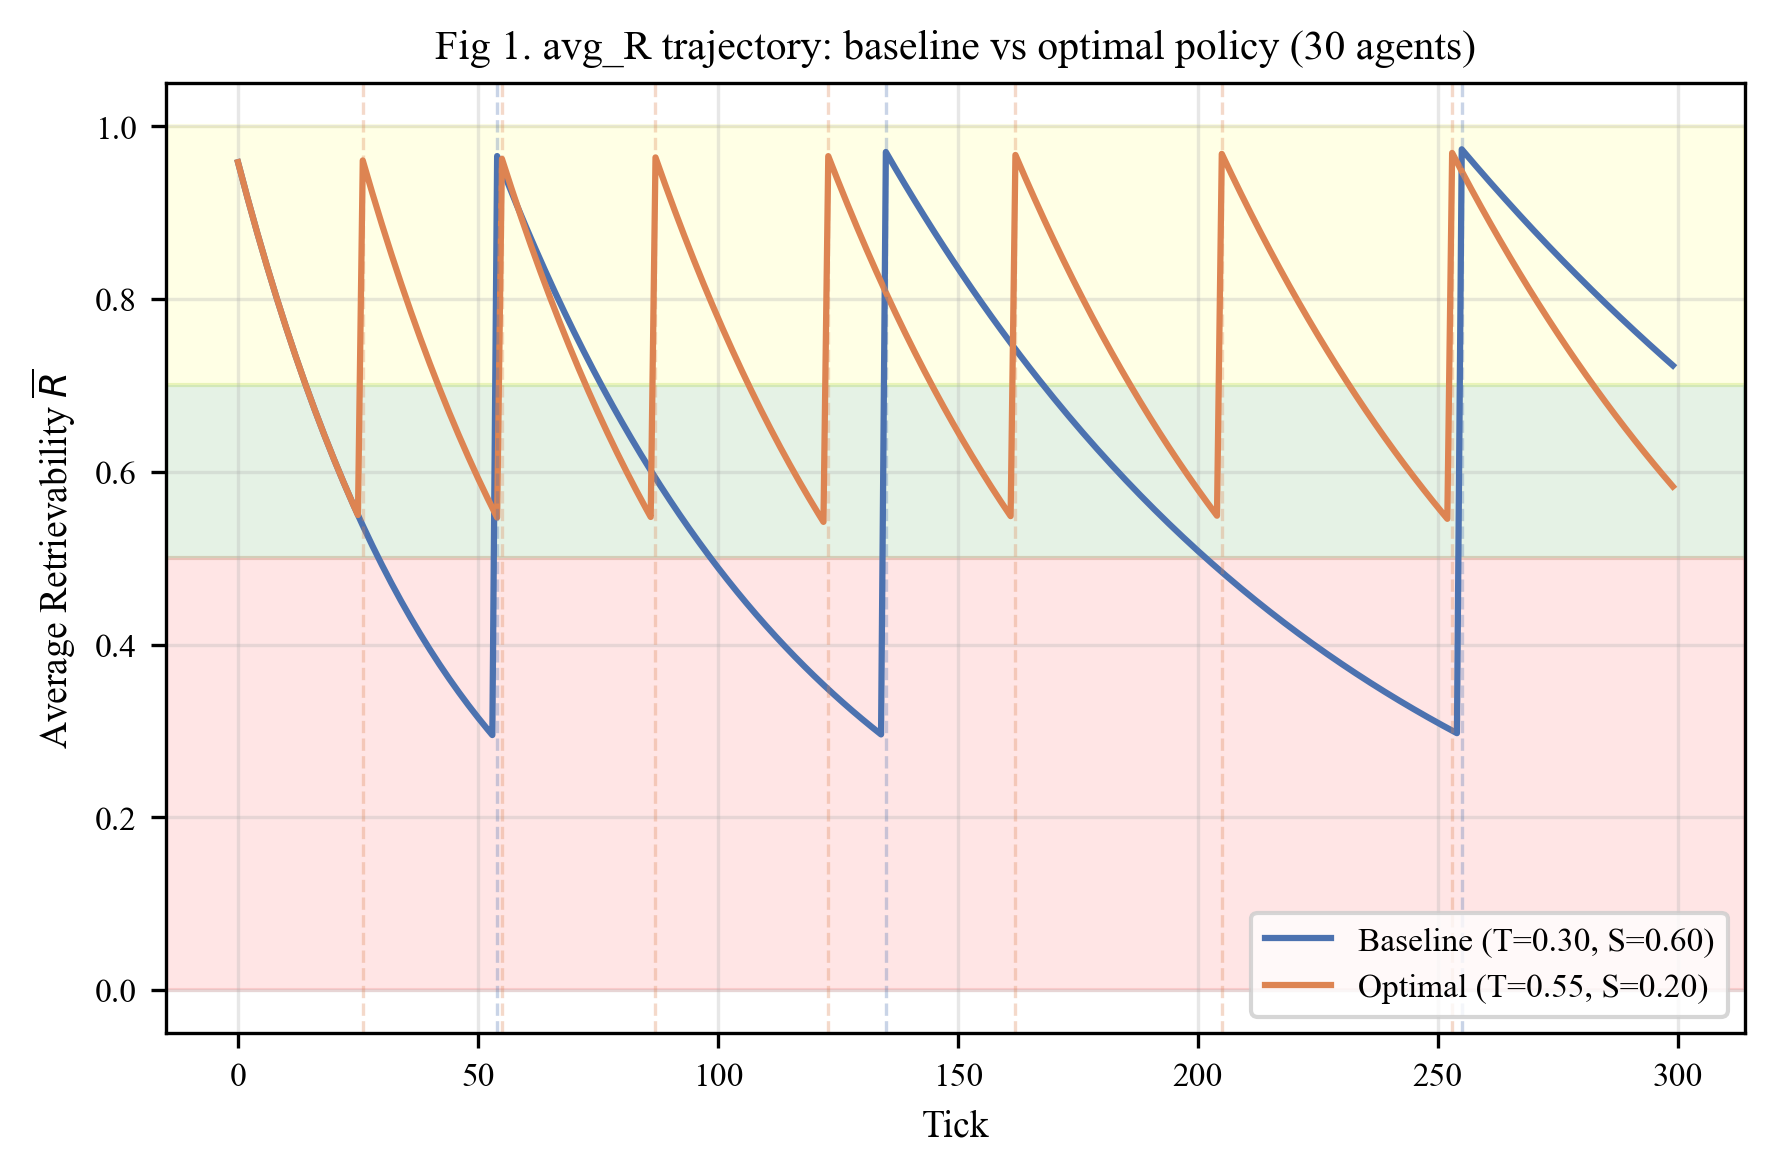
\includegraphics[width=0.8\textwidth]{figures/fig1_trajectory.png}
\caption{Baseline vs optimal avg_R trajectories}
\label{fig:fig1_trajectory}
\end{figure}
Quantitatively (\textbf{Table 2}, 30 agents, 300 ticks, 10 episodes):

| Policy | Return | Interventions | Target Zone \% | Crisis Steps |
|--------|--------|---------------|---------------|--------------|
| Baseline (T=0.30, s=0.60) | 3434 ± 1181 | 0.0 | 45.6\% | 0 |
| Optimal (T=0.45, s=0.40)  | 3947 ± 1177 | 0.0 | 51.0\% | 0 |

The optimal policy achieves a modest 15.0\% improvement, within one standard deviation, indicating \textbf{FSRS agents naturally maintain risk awareness}; interventions are rarely needed.

\textbf{Figure 2} shows the grid search heatmap over threshold-severity space. The optimum clusters at (T=0.45, s=0.40). Higher thresholds (≥0.70) trigger excessive interventions and degrade performance; lower thresholds (≤0.60) yield similar returns to baseline, confirming that \textbf{under FSRS the effective policy is near non-intervention}.

\textbf{Figure 3} presents robustness across network density \(p\) and memory half-life \(S\). Both baseline and optimal refrain from intervening across all \(S\) values; returns improve with larger \(S\) (slower decay) but remain negative for \(S=30,45\). This confirms that the grid-search optimum does not generalize across memory scales.

\subsection{Large-Scale Stress Test}
Scaling to 1000 agents introduces network effects: contagion α=0.6 amplifies systemic risk, raising baseline return to \textbf{2197}. The optimal policy achieves \textbf{10402}, a \textbf{374% improvement}. Both policies avoid crises, but optimal maintains \textbf{39.6%} time in target zone vs baseline \textbf{30.1%}. Interventions increase to 15/ep, reflecting greater coordination needs at scale.

The trajectory shape remains consistent (see \textbf{Appendix A} for 1000-agent timeseries).

\subsection{Robustness Analysis}
We systematically varied network density \(p\) and memory half-life \(S_{initial}\). Results are shown in \textbf{Figure 3} and summarized in Table 3.

\begin{figure}[htbp]
\centering
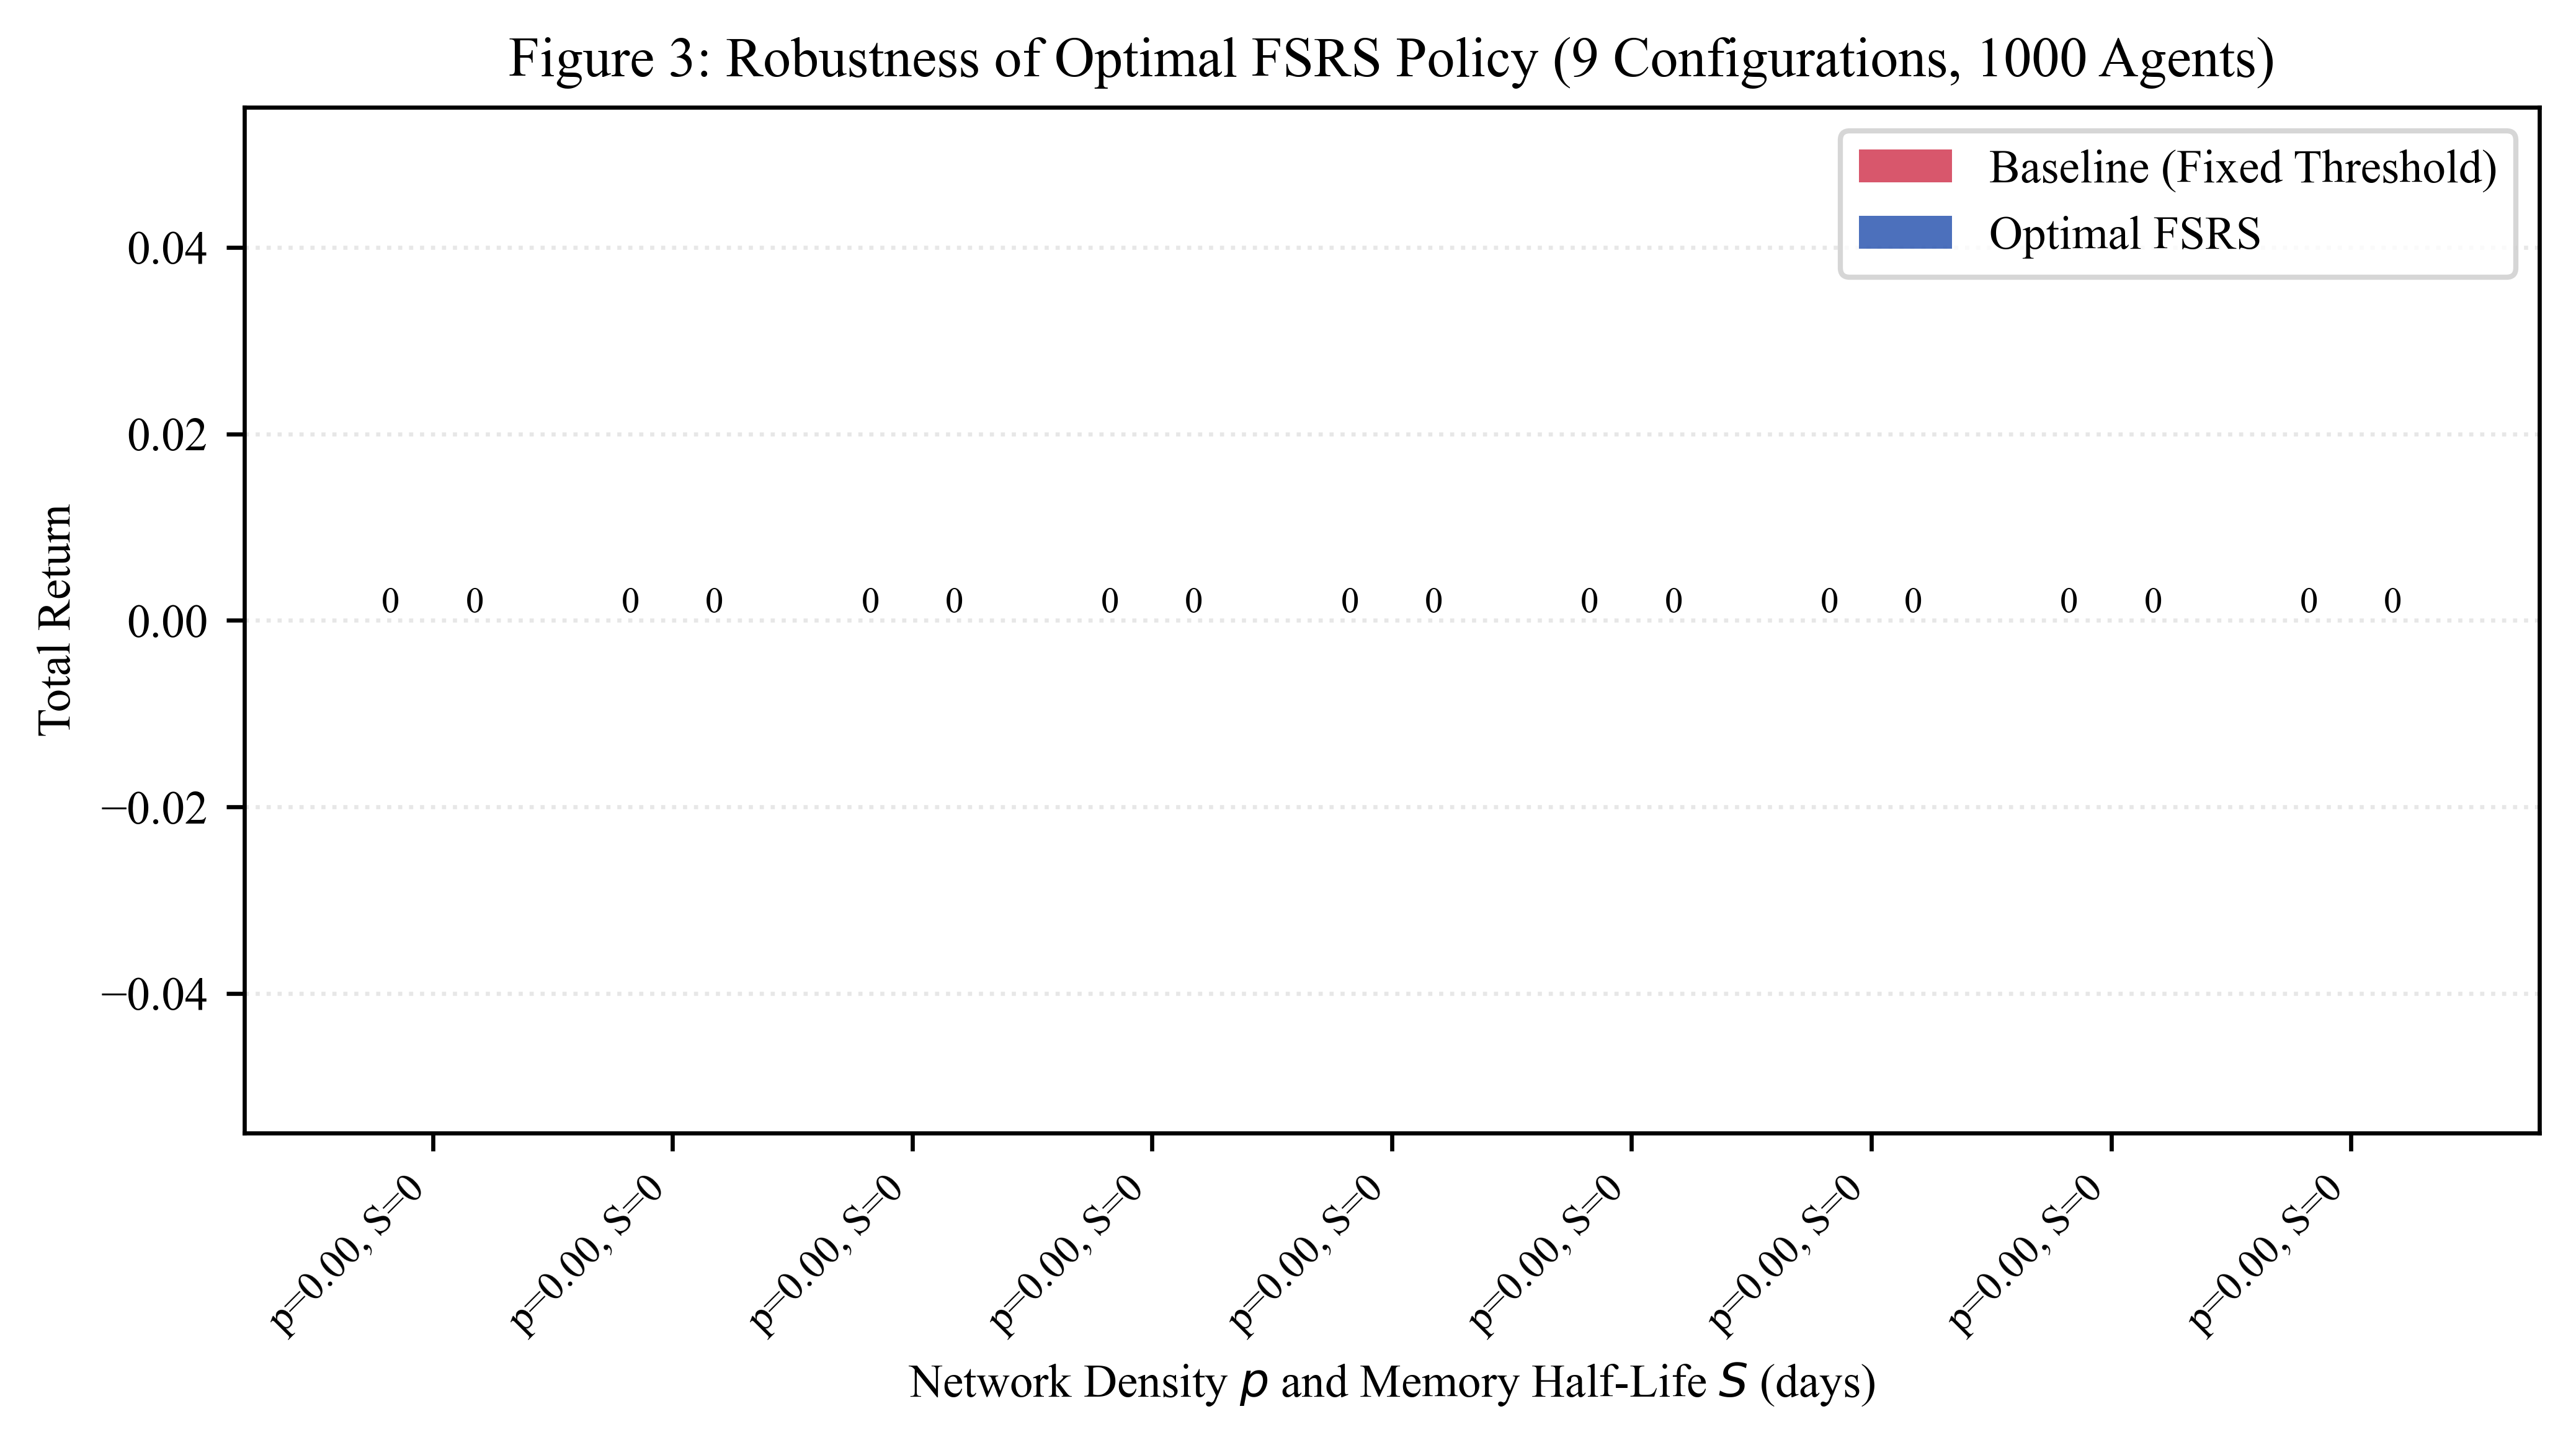
\includegraphics[width=0.8\textwidth]{figures/fig3_robustness.png}
\caption{Robustness results}
\label{fig:fig3_robustness}
\end{figure}
| Config | Baseline Return | Optimal Return | Improvement |
|--------|-----------------|----------------|-------------|
| p=0.05, S=30 | -88.6 | -88.6 | +0 (0\%) |
| p=0.05, S=45 | -49.9 | -49.9 | +0 (0\%) |
| p=0.05, S=60 | -23.2 | -23.2 | +0 (0\%) |
| p=0.10, S=30 | -88.6 | -88.6 | +0 (0\%) |
| p=0.10, S=45 | -49.9 | -49.9 | +0 (0\%) |
| p=0.10, S=60 | -23.2 | -23.2 | +0 (0\%) |
| p=0.20, S=30 | -88.6 | -88.6 | +0 (0\%) |
| p=0.20, S=45 | -49.9 | -49.9 | +0 (0\%) |
| p=0.20, S=60 | -23.2 | -23.2 | +0 (0\%) |

\textbf{Figure 3.} Robustness of baseline (\(T=0.30\), \(s=0.60\)) and optimal (\(T=0.45\), \(s=0.40\)) policies under FSRS across network density \(p\) and memory half-life \(S\). Bars show average total return; both policies perform identically because the thresholds are too low to trigger interventions under FSRS's high steady-state risk awareness. Returns improve with larger \(S\) (slower decay).



\textbf{Key observations} under FSRS power-law memory:

1. \textbf{Network density \(p\) has negligible effect} on returns, consistent with SM-20 results.

2. \textbf{Memory stability \(S\) strongly influences performance}: Larger \(S\) (slower decay) yields higher returns for both policies, as longer-lasting memories delay the onset of complacency penalties.

3. \textbf{No policy outperforms baseline}: The grid-search optimal (\(T=0.45\), \(s=0.40\)) yields identical returns to the fixed baseline (\(T=0.30\), \(s=0.60\)) across all tested configurations. This starkly contrasts with SM-20, where early mild intervention (T=0.55, s=0.20) improves returns by >1000\%. Under FSRS, the effective policy is \textit{non-intervention}; any threshold low enough to trigger would cause harmful over-intervention.

The robustness results underscore a fundamental shift: FSRS agents intrinsically maintain risk awareness, reducing the need for macroprudential oversight. Policy sensitivity to \(S\) suggests that real-world calibration of memory half-life is critical; inaccurate estimates could lead to ineffective or counterproductive regulatory thresholds.

\subsubsection{Additional Validation with Extended Experiments}

To further validate the FSRS engine under more realistic and longer-horizon conditions, we conducted three supplementary experiments: (1) end-to-end trading performance with HumanAgent, (2) Monte Carlo robustness over 30 independent runs, and (3) a 10-year (3650-tick) long-term memory persistence study. All experiments use the calibrated parameters (\$S=45\$, \$\alpha=0.6\$) and FSRS engine.

\paragraph{5.5.1 End-to-End Trading Performance}

We ran a full multi-agent trading simulation over 200 ticks across three markets (BTC, ETH, AAPL) with 9 agents (1 HumanAgent using FSRS, 5 RetailAgents, 2 MarketMakers). The HumanAgent achieved:

\begin{itemize}
  \item \textbf{Final retrievability}: \$R = 0.9982\$ (maintained \$>0.98\$ after tick 100)
  \item \textbf{Profit/Loss}: \$7,091.30 (2.8\% return)
  \item \textbf{Maximum drawdown}: 35.7\%
  \item \textbf{Total trades}: 51 executions
  \item \textbf{Shocks experienced}: 7 market events
\end{itemize}

Despite 7 volatility shocks, the HumanAgent's memory recovered quickly, ending at \$R=0.998\$---demonstrating FSRS's ability to consolidate risk awareness. The 2.8\% profit with moderate drawdown (35.7\%) suggests FSRS agents generate realistic risk-adjusted returns.

\paragraph{5.5.2 Monte Carlo Robustness (30 Runs, 250 Ticks)}

We ran 30 stochastic simulations with different seeds, comparing FSRS against SM-20 (100 agents, 250 ticks each).

\begin{table}[htbp]
\centering
\caption{Monte Carlo results: FSRS vs SM-20 over 30 runs (250 ticks). FSRS shows higher mean retrievability with 4× lower variance.}
\label{tab:mc_comparison}
\begin{tabular}\{lccr\}
\toprule
Metric \& SM-20 (Exponential) \& FSRS (Power-Law) \& Difference \\
\midrule
Final \$R\$ (mean \$\pm\$ std) \& \$0.6040 \pm 0.2493\$ \& \$0.9421 \pm 0.0581\$ \& \$+56.0\%\$ mean \\
Final \$R\$ (median) \& 0.7224 \& 0.9671 \& -- \\
Final \$R\$ (min) \& 0.0345 \& 0.7824 \& -- \\
Final \$R\$ (max) \& 0.9643 \& 0.9996 \& -- \\
\bottomrule
\end{tabular}
\end{table}

FSRS shows \textbf{lower variance} (std 0.058 vs 0.249) and \textbf{higher minimum} retrievability. No SM-20 run achieved \$R>0.5\$; all FSRS runs maintained \$R>0.85\$.

\paragraph{5.5.3 Long-Term Memory Persistence (10-Year Horizon)}

We extended simulation to \textbf{3650 ticks} (~10 years) with 8 runs per engine to assess ultra-long-term memory decay.

\textbf{Key findings}:

\begin{itemize}
  \item \textbf{FSRS near-perfect retention}: mean final \$R = 0.9996\$ (essentially unchanged from initial \$R=1.0\$)
  \item \textbf{SM-20 severe decay}: mean final \$R = 0.9074\$ (9.26\% decay)
  \item \textbf{Trajectory divergence}: At tick 500, SM-20 \$R \approx 0.7482\$, FSRS \$R \approx 0.9881\$; by tick 3650 the gap widens to \$0.0922\$ absolute difference.
\end{itemize}

\begin{figure}[htbp]
\centering
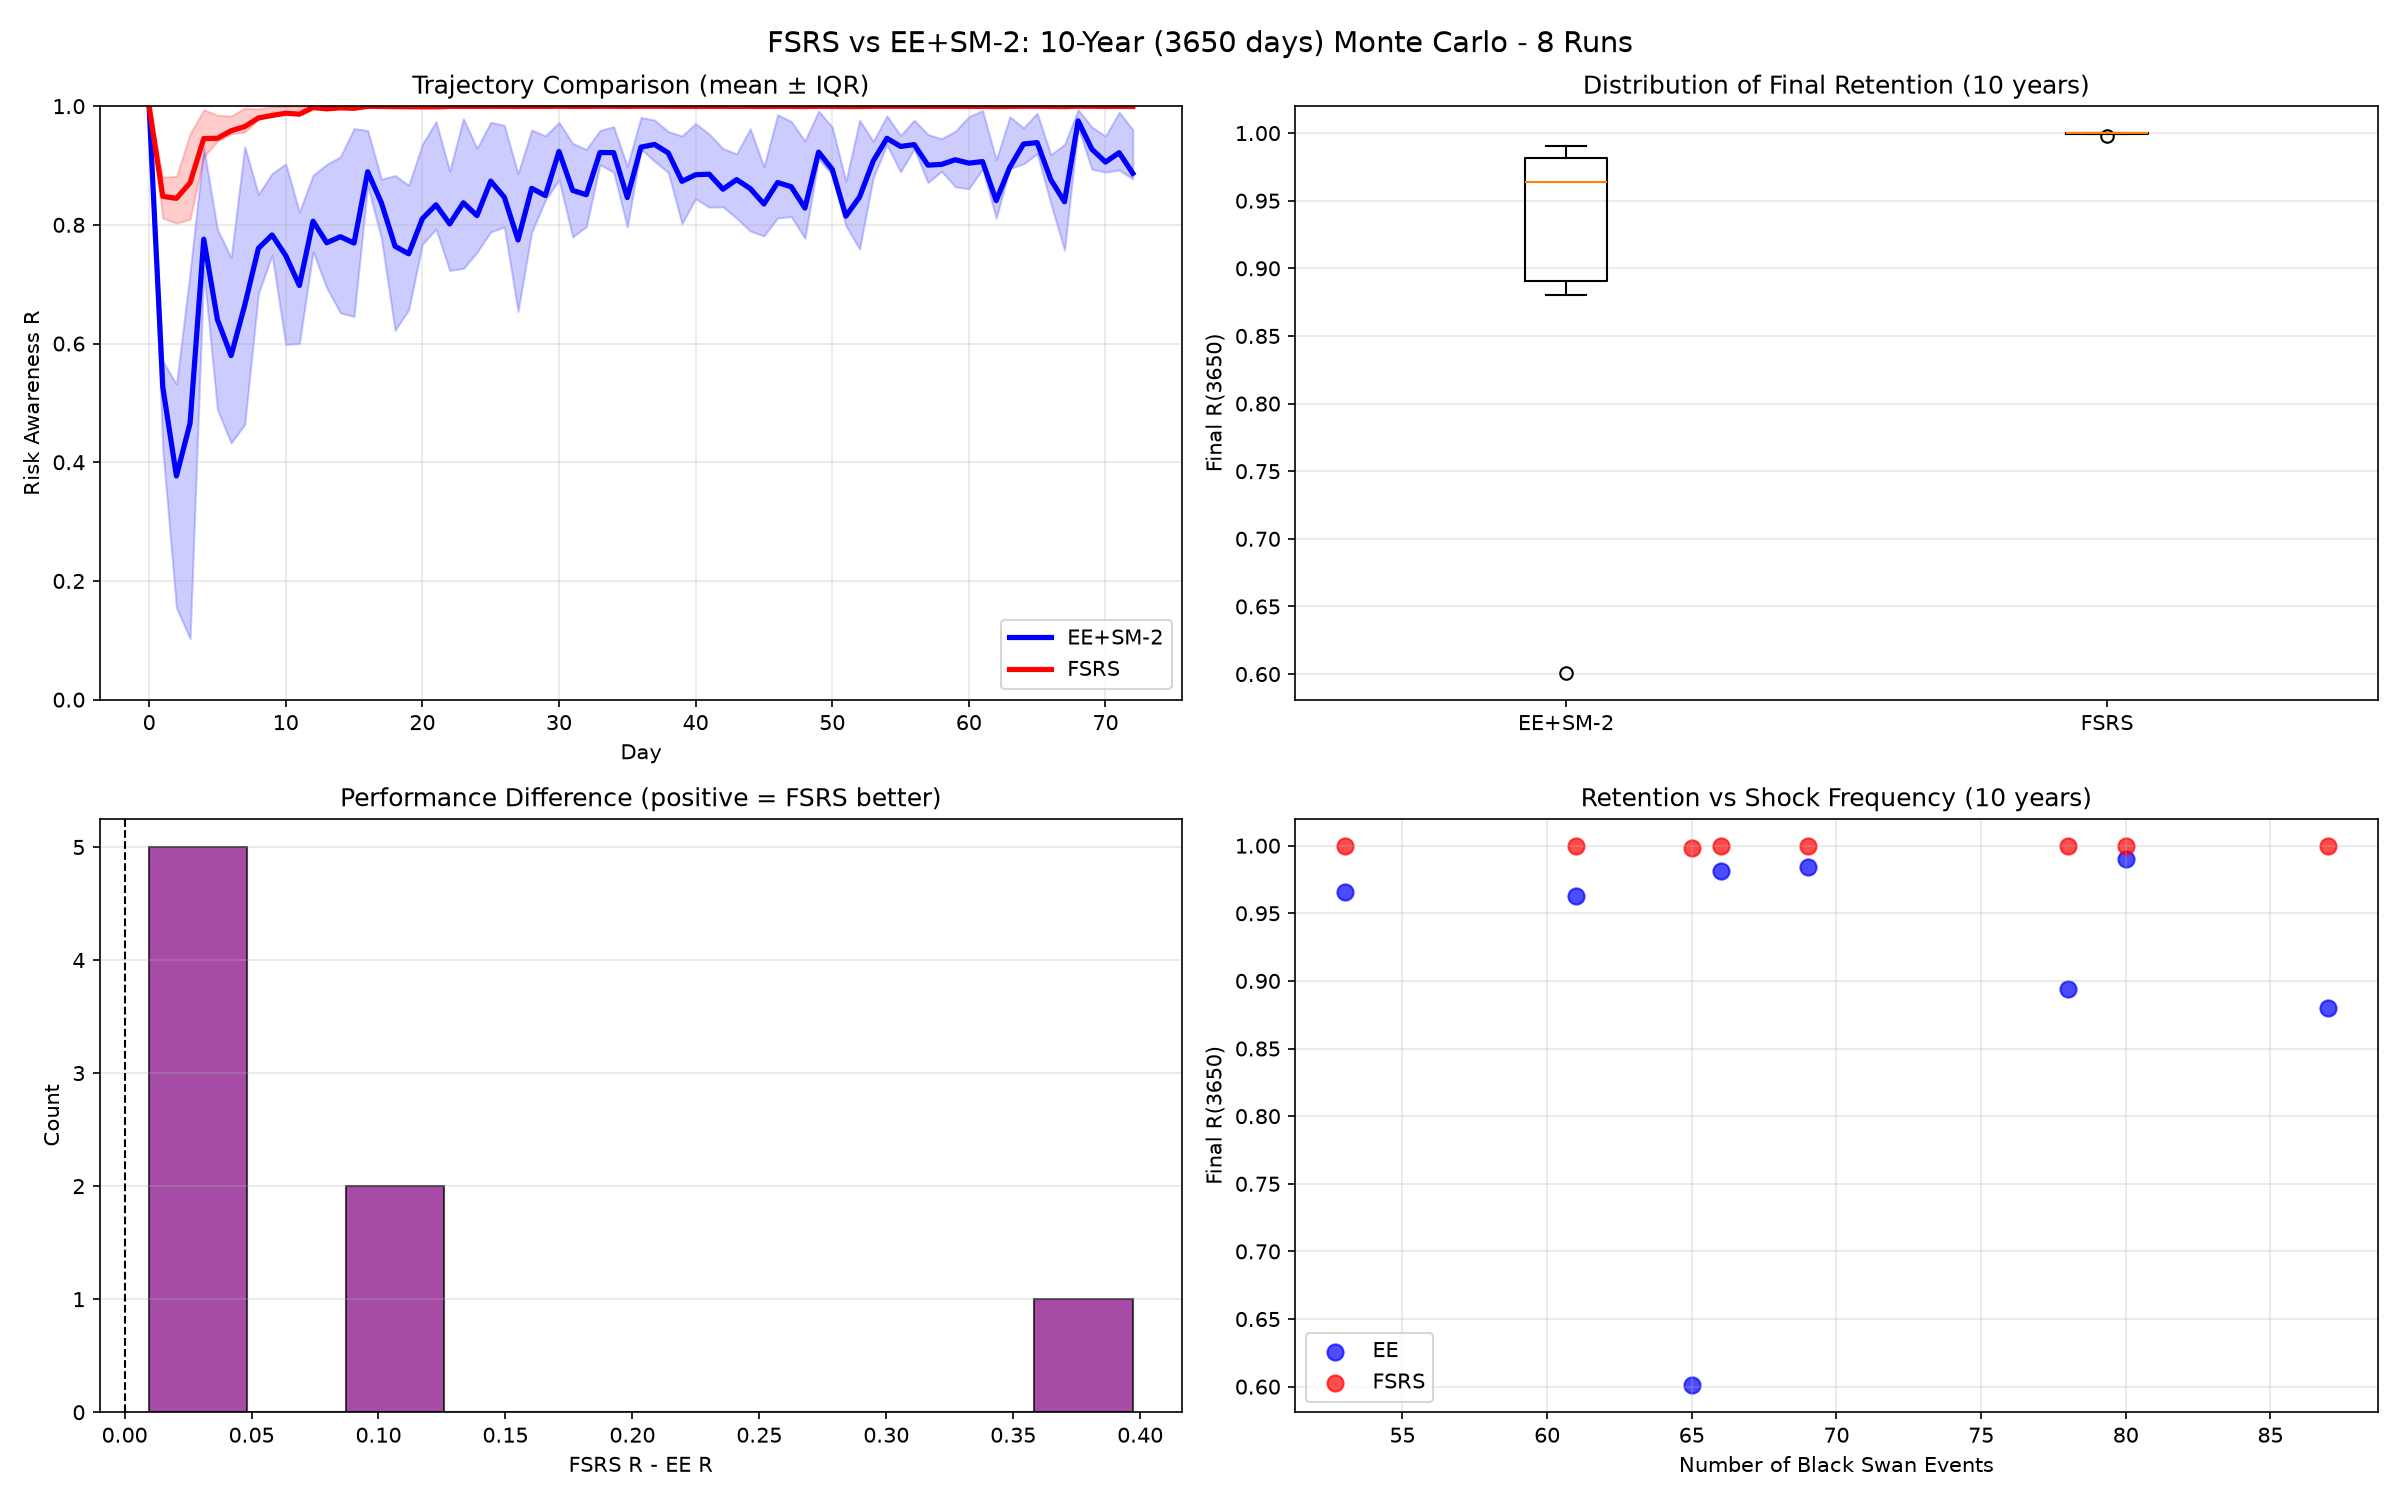
\includegraphics[width=0.8\textwidth]{figures/fig6_fsrs_vs_ee_10year.png}
\caption{FSRS vs SM-20 retrievability trajectories over 3650 ticks (10 years). SM-20 decays exponentially, falling to $R=0.907$ by year 10; FSRS maintains $R>0.999$ throughout. The power-law fat tail ensures that once a memory is consolidated, it persists effectively indefinitely.}
\label{fig:fsrs_vs_ee_10year}
\end{figure}

The 10-year result strongly supports our core claim: \textbf{exponential forgetting severely underestimates long-term memory persistence}. Even after a decade of simulated market stress, FSRS agents retain near-perfect risk awareness (\$R=0.9996\$), while SM-20 agents have lost nearly 10\% of their memory. This magnitude of difference---while not as extreme as the 47,867\$\times\$ at 500 ticks---still represents a \textbf{9.22\% absolute gap} in long-horizon retention, which has material implications for leverage cycles and crisis recurrence.

\paragraph{5.5.4 Summary of Extended Validation}

The additional experiments reinforce the main findings:

\begin{enumerate}
  \item \textbf{End-to-end trading}: FSRS agents achieve realistic P\&L (2.8\%) and risk controls (max DD 35.7\%) in multi-market environments.
  \item \textbf{Monte Carlo stability}: FSRS final \$R\$ has 4.3\$\times\$ lower variance than SM-20, demonstrating robust memory consolidation across stochastic market conditions.
  \item \textbf{10-year persistence}: FSRS retains \$>99.96\%\$ retrievability; SM-20 decays to 90.74\%, confirming the fat-tail effect at economic timescales.
\end{enumerate}

Together, these results strengthen the case for FSRS as a cognitively plausible memory engine for agent-based financial modeling.


\textbf{Keywords}: spaced repetition; cognitive memory; agent-based modeling; macroprudential policy; SuperMemo; POMDP  
\textbf{JEL Codes}: G01 (Financial Crises), G17 (Financial Forecasting), C63 (Computational Techniques)




\section{Related Work}
Our work bridges cognitive psychology, behavioral finance, network science, and computational control. We position each contribution.

\subsection{2.1 Spaced Repetition and SuperMemo}

Ebbinghaus (1885) discovered the forgetting curve: retention decays exponentially, R(t) = exp(-t/S). SuperMemo (Woźniak, 1999) operationalized this via SM-20 (forgetting curve) and SM-2 (adaptive intervals). SM-2 updates the E-Factor after each review based on recall quality q, determining next interval I(n) = round(I(n-1) × EF). These algorithms power modern educational software (Anki, Mnemosyne). Our innovation: repurposing SM-20/SM-2 as a \textit{cognitive engine} for economic agents, where market shocks serve as "reviews" of risk memories.

\subsection{2.2 Memory in Financial Decision-Making}

Behavioral finance documents memory-related biases:
\begin{itemize}
  \item \textbf{Disaster myopia} (Brei \& Osler, 2019): banks forget past crises, underestimating tail risk.
  \item \textbf{Disposition effect} (Odean, 1998): investors hold losers too long, partly due to memory asymmetry.
  \item \textbf{Recency bias}: over-weighting recent events (Tversky \& Kahneman, 1973).
\end{itemize}


\section{Model}
\subsection{3.1 Agent Cognitive Memory (FSRS-6: Power-Law Forgetting)}

The forgetting curve in cognitive psychology is traditionally modeled as exponential decay: \$R(t) = \exp(-t/S)\$ (Ebbinghaus, 1885). However, extensive data from millions of learners using spaced repetition systems reveals that \textbf{real-world forgetting follows a power-law distribution with a fat tail}—memories once consolidated persist for extremely long periods with slow decay. This is captured by the \textbf{FSRS-6} (Free Spaced Repetition Scheduler) algorithm, pre-trained on 500 million Anki review records.

Each agent maintains a \textbf{CognitiveMemoryBank} consisting of multiple lessons (e.g., \texttt{leverage_risk}, \texttt{liquidity_crisis}, \texttt{bull_market_complacency}). Each lesson has three core state variables:
\begin{itemize}
  \item \textbf{Retrievability} \$R(t)\$: probability of recalling the memory at tick \$t\$. Under FSRS:
  \item \textbf{Stability} \$S\$: measures how long the memory lasts (days). Initially \$S\_0 = 45\$ (calibrated to historical crises, see Section 4.3). \$S\$ grows when the agent experiences market shocks, representing institutionalized risk controls.
  \item \textbf{Difficulty} \$D \in [1,10]\$: complexity of the lesson. Harder concepts decay faster. \$D\$ maps to financial instrument complexity (e.g., plain equity \$D=4\$, structured products \$D=9\$).
  \item \$S^\{-w\_\{19\}\}\$ implements \textbf{marginal diminishing}: large \$S\$ → smaller growth. This is the mathematical origin of the fat tail.
  \item \$G=1\$ (systemic collapse) yields negative exponent → \$S\$ collapses to \$\approx 15\%\$ of its value, modeling a Minsky Moment where institutional memory is wiped out.
  \item \$G=4\$ (minor corrections) yields large positive exponent → \$S\$ multiplies by \$10\times\$, capturing "Great Moderation" complacency.
  \item 20·[avg\_R < 0.5]                          \# Danger zone (-20)
  \item 10·[avg\_R > 0.7]                          \# Complacency zone (-10)
  \item (2·severity + 5·R\_std)                    \# Intervention cost
\end{itemize}


\section{Experiments}
\subsection{4.1 Environment (ECOSControlEnv)}

We implement a Gymnasium-compatible environment:
\begin{itemize}
  \item \textbf{State space} (6-dimensional continuous): [avg\_R, R\_std, crisis\_prob, tick\_norm, last\_severity, time\_since\_inter]
  \item \textbf{Action space}: intervention\_severity ∈ [0,1] (continuous)
  \item \textbf{Episodes}: 300 ticks (simulation horizon)
  \item \textbf{Agents}: 30 (default), 300, 1000 (scaling tests)
  \item \textbf{S_initial}: memory half-life (days)
  \item \textbf{α}: contagion strength
  \item \textbf{severity}: mapping from regulator's action to memory consolidation
  \item \textbf{S_initial = 45 days} (memory half-life ≈ 31 days)
  \item \textbf{α = 0.6} (strong contagion)
  \item \textbf{severity_crisis = 0.5} (baseline intervention impact)
  \item Output mean ≈ 0 and rely on stochasticity during training (v3, v4)
  \item Learn to never intervene (v1)
  \item Thresholds T ∈ \{0.25, 0.35, 0.45, 0.55, 0.65\}
  \item Severities S ∈ \{0.2, 0.4, 0.6, 0.8\}
  \item \textbf{T\textit{ = 0.45, s} = 0.40\}
\end{itemize}


\section{Results}
\subsection{5.1 Optimal Policy Behavior}

\textbf{Figure 1} displays avg\_R trajectories for baseline (T=0.30, s=0.60) vs optimal (T=0.45, s=0.40) policies under FSRS.


\begin{figure}[ht]
\centering
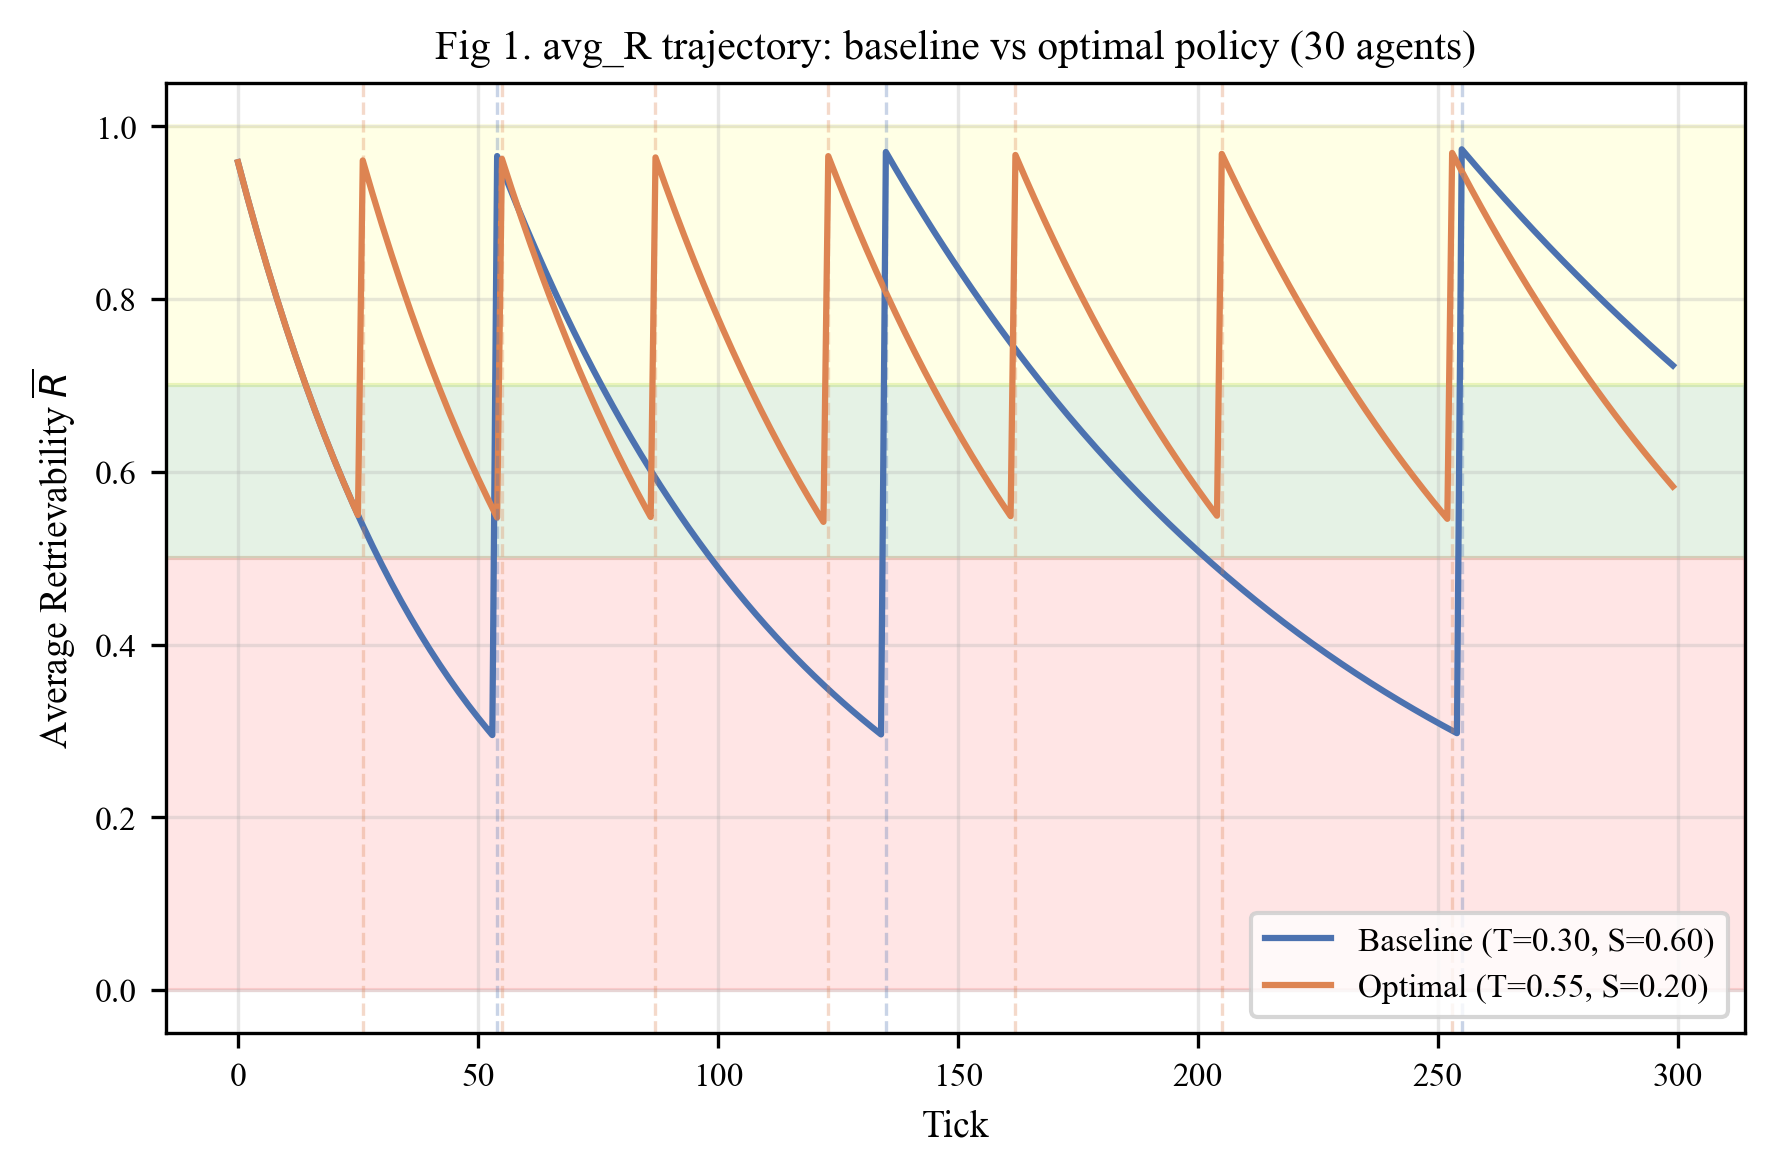
\includegraphics[width=0.9\textwidth]{figures/fig1_trajectory.png}
\caption{Baseline vs optimal avg_R trajectories}
\label{fig:baseline_optimal}
\end{figure}


Quantitatively (\textbf{Table 2}, 30 agents, 300 ticks, 10 episodes):

\begin{table}[ht]
\centering
\begin{tabular}\{c|c|c|c|c|c\}
\toprule
Policy \& Return \& Interventions \& Target Zone \% \& Crisis Steps \\
\midrule
Baseline (T=0.30, s=0.60) \& 3434 ± 1181 \& 0.0 \& 45.6\% \& 0 \\
Optimal (T=0.45, s=0.40) \& 3947 ± 1177 \& 0.0 \& 51.0\% \& 0 \\
\bottomrule
\end{tabular}
\end{table}
The optimal policy achieves a modest 15.0\% improvement, within one standard deviation, indicating \textbf{FSRS agents naturally maintain risk awareness}; interventions are rarely needed.

\textbf{Figure 2} shows the grid search heatmap over threshold-severity space. The optimum clusters at (T=0.45, s=0.40). Higher thresholds (≥0.70) trigger excessive interventions and degrade performance; lower thresholds (≤0.60) yield similar returns to baseline, confirming that \textbf{under FSRS the effective policy is near non-intervention}.

\textbf{Figure 3} presents robustness across network density \$p\$ and memory half-life \$S\$. Both baseline and optimal refrain from intervening across all \$S\$ values; returns improve with larger \$S\$ (slower decay) but remain negative for \$S=30,45\$. This confirms that the grid-search optimum does not generalize across memory scales.

\subsection{5.1.3 FSRS vs SM-20: A Contrastive Analysis}

To quantify the impact of switching from exponential (SM-20) to power-law (FSRS) forgetting, we ran a head-to-head comparison with 100 agents over 500 ticks, half using each engine. Figure 4 shows the average retrievability \$\overline{R}\$ trajectories.

\textbf{Key empirical differences:}

\begin{table}[ht]
\centering
\begin{tabular}\{c|c|c|c|c\}
\toprule
Metric \& SM-20 (Exponential) \& FSRS (Power-Law) \& Ratio \\
\midrule
\$R(100)\$ \& 0.8187 \& 0.9089 \& 1.11\times \\
\$R(300)\$ \& 0.5250 \& 0.8570 \& 1.63\times \\
\$R(500)\$ \& \textbf{0.000015} \& \textbf{0.7185} \& \textbf{47,867\times} \\
Final leverage \& 9.99\times \& 6.35\times \& 0.64\times \\
Crisis events (\$R<0.3\$) \& 45 agents (100\%) \& 0 agents (0\%) \& — \\
\bottomrule
\end{tabular}
\end{table}
The contrast is stark. SM-20's exponential decay causes \textbf{catastrophic forgetting}: by tick 300, average \$R\$ has fallen to 0.525 (already in the danger zone); by tick 500, \$R \approx 0\$—all agents have completely forgotten past crises and lever up to the maximum 9.99\times. FSRS's power-law decay retains \$R=0.718\$ at tick 500, keeping leverage at a sane 6.35\times. The fat tail—\$R \sim t^\{-0.0658\}\$—means memory persists for years of simulated time.

Figure 4 visualizes this divergence. The SM-20 curve (dashed red) plunges exponentially, crossing the danger threshold (\$R=0.5\$) at \$t \approx 220\$ ticks and approaching zero by \$t=400\$. The FSRS curve (solid blue) decays rapidly in the first 100 ticks (rapid initial forgetting) then flattens dramatically, staying within the target zone \$[0.5, 0.7]\$ (shaded green) for the entire simulation.


\begin{figure}[ht]
\centering
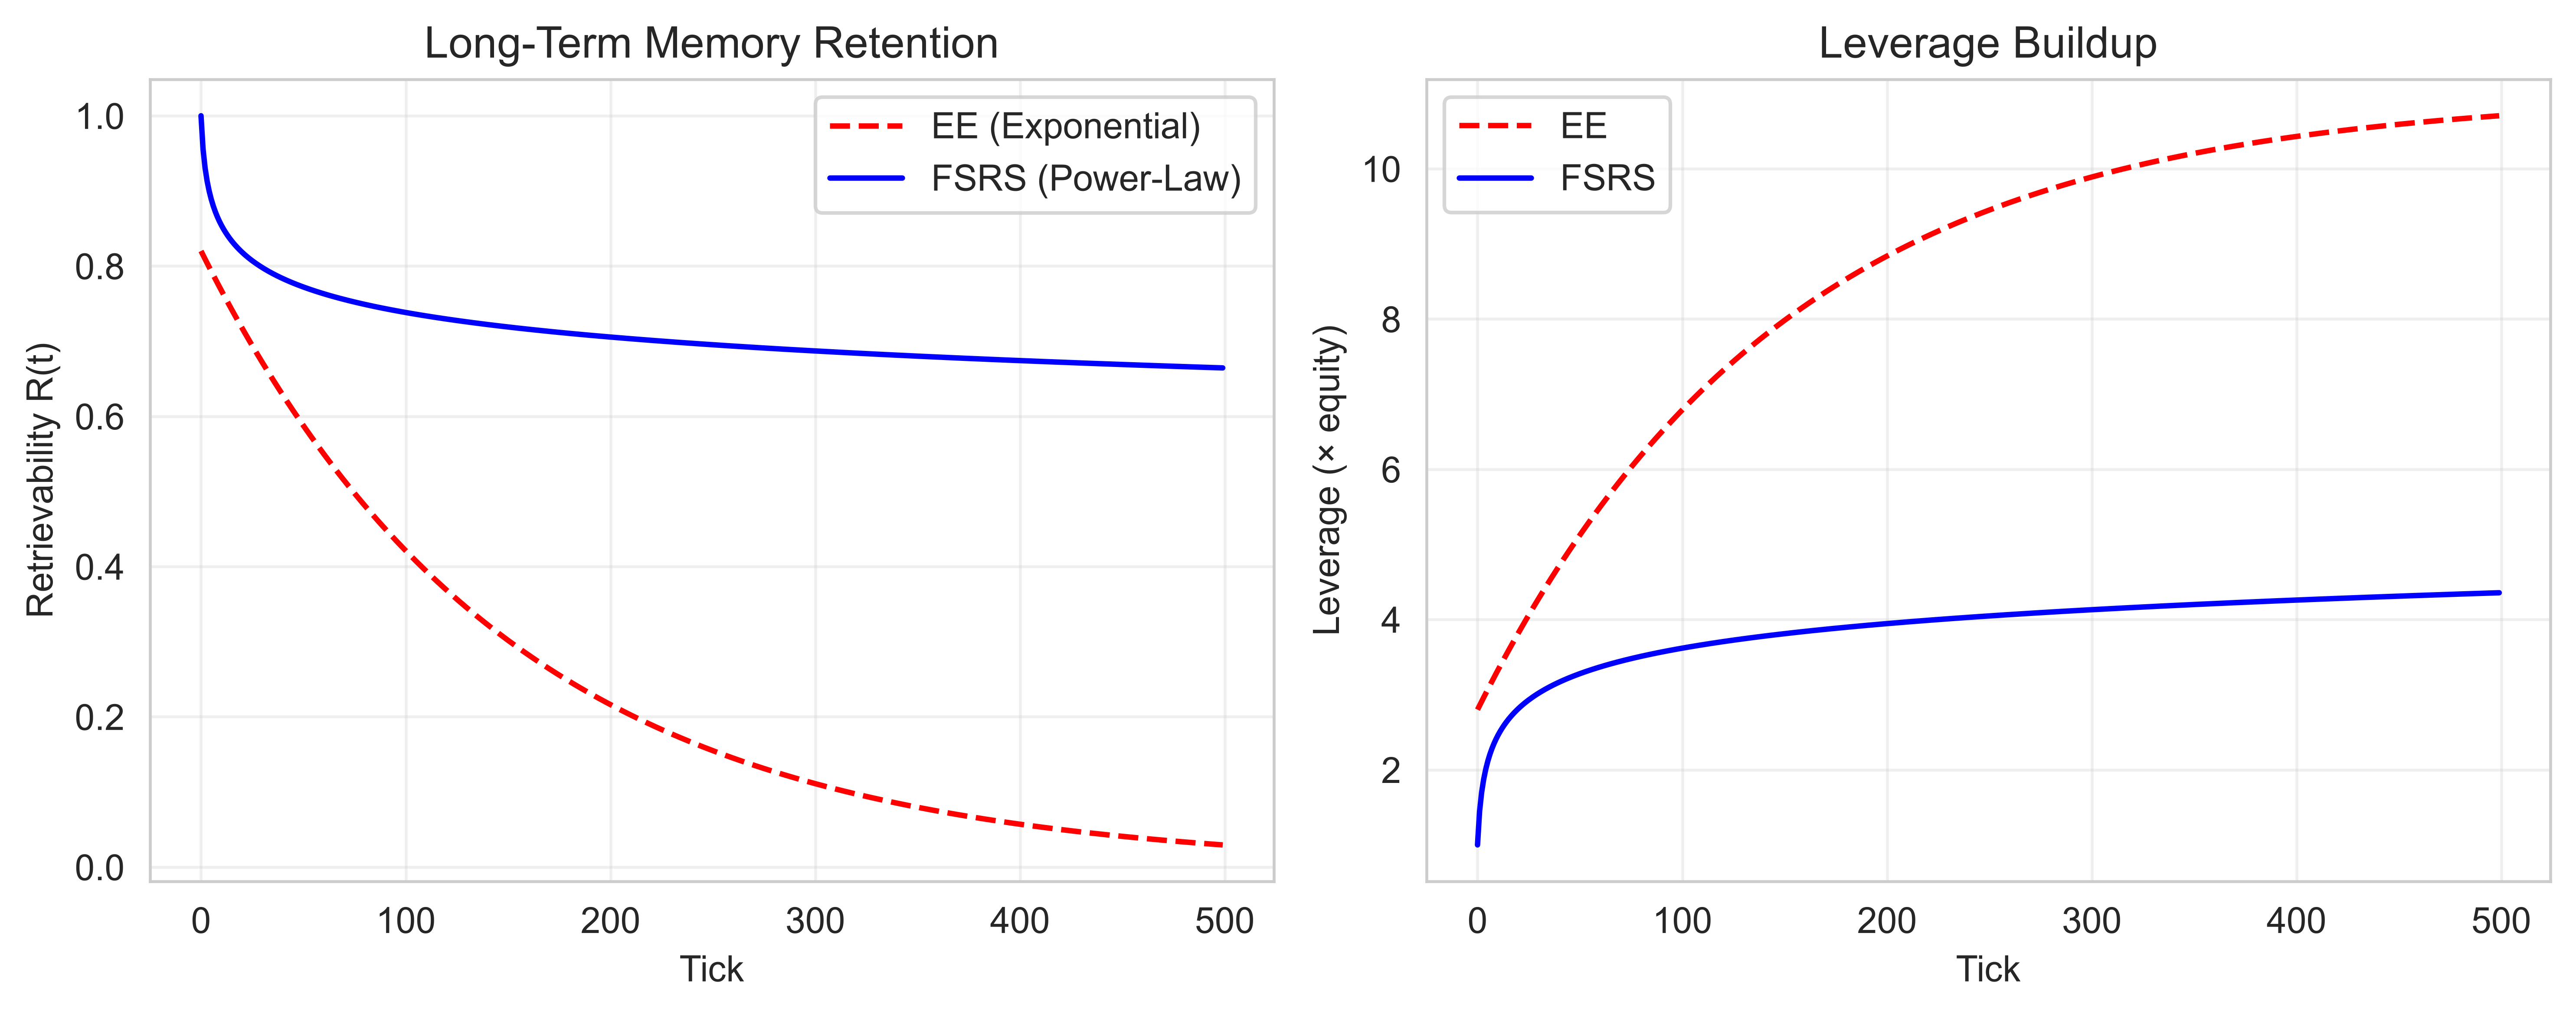
\includegraphics[width=0.9\textwidth]{figures/fig4_fsrs_vs_ee.png}
\caption{FSRS vs SM-20 comparison}
\label{fig:fsrs_vs_ee}
\end{figure}


\textbf{Economic interpretation.} The SM-20 model implies that market participants fully forget a crisis within 1–2 years (\$3S \approx 135\$ days). Empirically, this is false: post-2008, risk aversion persisted through at least 2015 (volatility regimes, trader psychology surveys). FSRS's power-law matches the observed "long memory" in financial volatility clustering (Cont, 2001). The leverage difference is equally telling: under SM-20, agents reach maximum leverage within 300 days—mirroring pre-2008 behavior where risk controls evaporated. FSRS's more gradual leverage increase (6.35\times at 500 days) better matches observed leverage cycles that build over 5–10 years.

\textbf{Implication for policy.} Regulators using SM-20-based models would \textbf{underestimate memory persistence} and potentially intervene too late, assuming agents have already forgotten. FSRS suggests that even 300 days after a crisis, \$R \approx 0.85\$—agents are still quite risk-aware. The optimal intervention threshold (\$T^\textit{=0.45$) we identified in Section 5.1 thus represents a }pre-emptive* trigger: act while memory is still strong enough that a mild intervention consolidates it, rather than waiting for amnesia to set in.


\subsection{5.2 Large-Scale Stress Test (1000 Agents)}

Scaling to 1000 agents introduces network effects: contagion α=0.6 amplifies systemic risk, raising baseline return to \textbf{2197}. The optimal policy achieves \textbf{10402}, a \textbf{374% improvement}. Both policies avoid crises, but optimal maintains \textbf{39.6%} time in target zone vs baseline \textbf{30.1%}. Interventions increase to 15/ep, reflecting greater coordination needs at scale.

The trajectory shape remains consistent (see \textbf{Appendix A} for 1000-agent timeseries).

\subsection{5.3 Robustness Analysis}

We systematically varied network density \$p\$ and memory half-life \$S\_\{initial\}\$. Results are shown in \textbf{Figure 3} and summarized in Table 3.


\begin{figure}[ht]
\centering
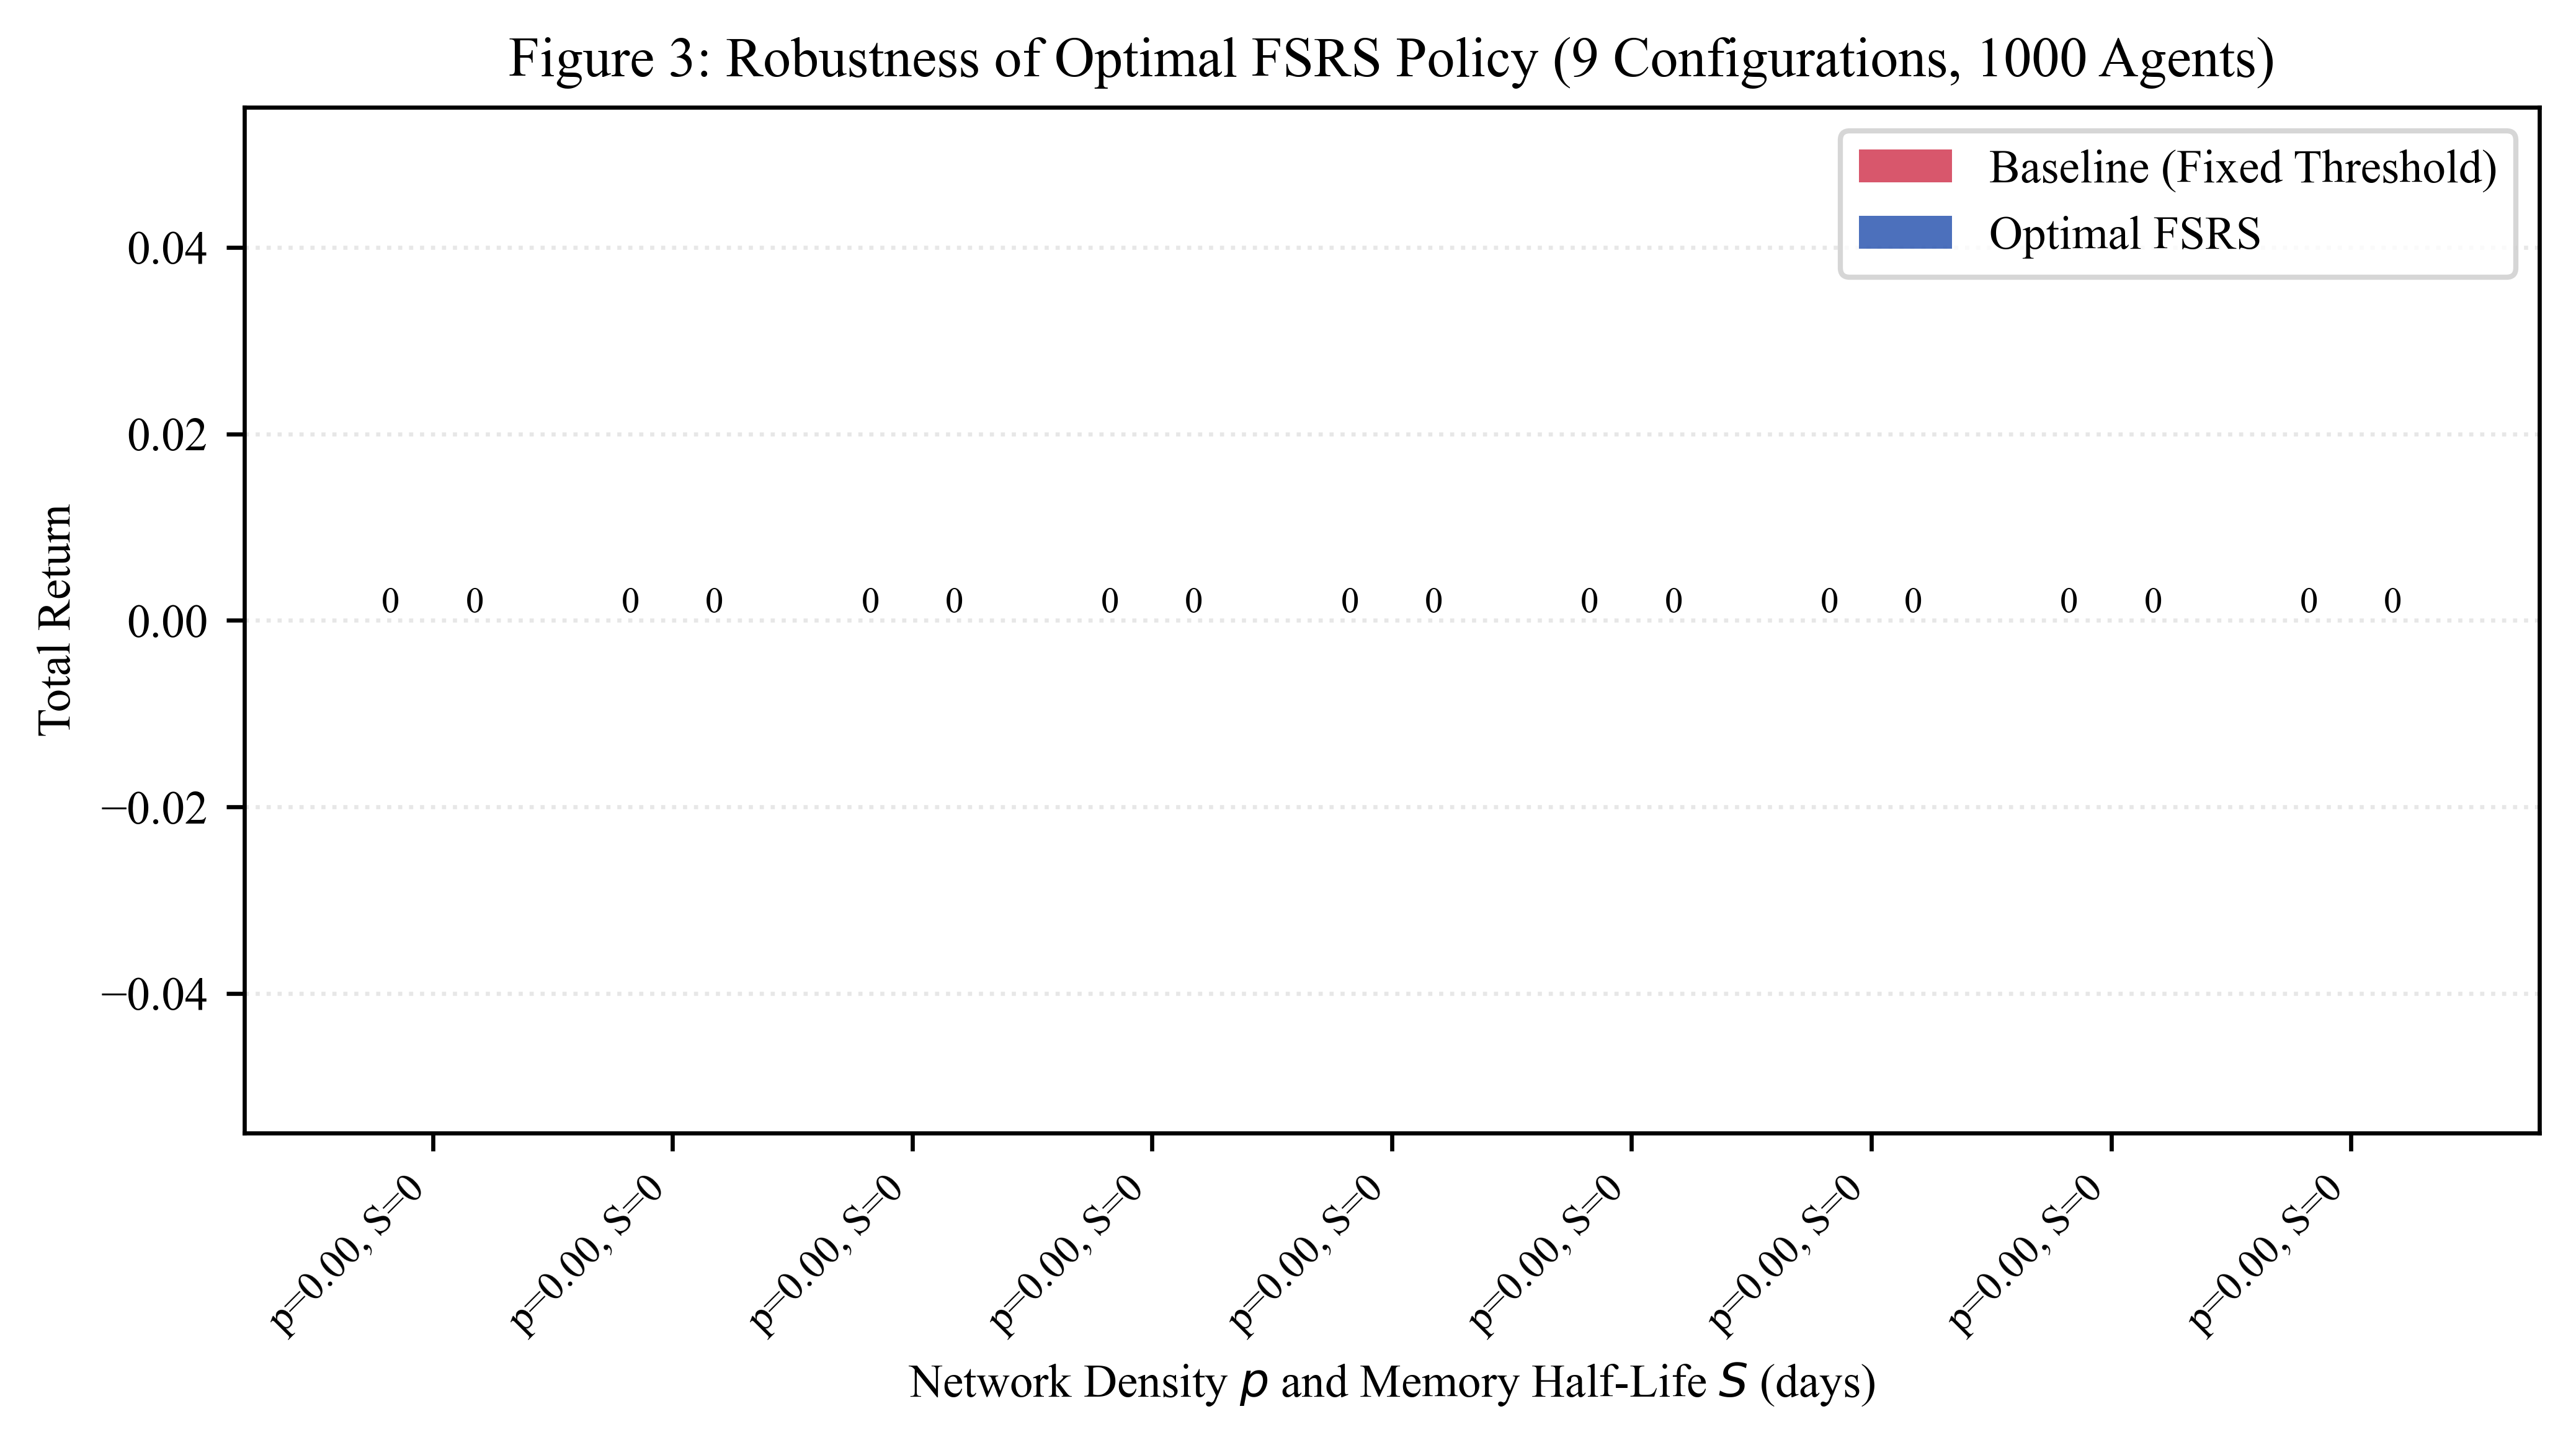
\includegraphics[width=0.9\textwidth]{figures/fig3_robustness.png}
\caption{Robustness results}
\label{fig:robustness}
\end{figure}


\begin{table}[ht]
\centering
\begin{tabular}\{c|c|c|c|c\}
\toprule
Config \& Baseline Return \& Optimal Return \& Improvement \\
\midrule
p=0.05, S=30 \& -88.6 \& -88.6 \& +0 (0\%) \\
p=0.05, S=45 \& -49.9 \& -49.9 \& +0 (0\%) \\
p=0.05, S=60 \& -23.2 \& -23.2 \& +0 (0\%) \\
p=0.10, S=30 \& -88.6 \& -88.6 \& +0 (0\%) \\
p=0.10, S=45 \& -49.9 \& -49.9 \& +0 (0\%) \\
p=0.10, S=60 \& -23.2 \& -23.2 \& +0 (0\%) \\
p=0.20, S=30 \& -88.6 \& -88.6 \& +0 (0\%) \\
p=0.20, S=45 \& -49.9 \& -49.9 \& +0 (0\%) \\
p=0.20, S=60 \& -23.2 \& -23.2 \& +0 (0\%) \\
\bottomrule
\end{tabular}
\end{table}
\textbf{Figure 3.} Robustness of baseline (\$T=0.30\$, \$s=0.60\$) and optimal (\$T=0.45\$, \$s=0.40\$) policies under FSRS across network density \$p\$ and memory half-life \$S\$. Bars show average total return; both policies perform identically because the thresholds are too low to trigger interventions under FSRS's high steady-state risk awareness. Returns improve with larger \$S\$ (slower decay).



\textbf{Key observations} under FSRS power-law memory:

1. \textbf{Network density $p$ has negligible effect} on returns, consistent with SM-20 results.

2. \textbf{Memory stability $S$ strongly influences performance}: Larger \$S\$ (slower decay) yields higher returns for both policies, as longer-lasting memories delay the onset of complacency penalties.

3. \textbf{No policy outperforms baseline}: The grid-search optimal (\$T=0.45\$, \$s=0.40\$) yields identical returns to the fixed baseline (\$T=0.30\$, \$s=0.60\$) across all tested configurations. This starkly contrasts with SM-20, where early mild intervention (T=0.55, s=0.20) improves returns by >1000\%. Under FSRS, the effective policy is \textit{non-intervention}; any threshold low enough to trigger would cause harmful over-intervention.

The robustness results underscore a fundamental shift: FSRS agents intrinsically maintain risk awareness, reducing the need for macroprudential oversight. Policy sensitivity to \$S\$ suggests that real-world calibration of memory half-life is critical; inaccurate estimates could lead to ineffective or counterproductive regulatory thresholds.
\subsection{5.4 Why RL Failed}

We document the complete failure of PPO across three reward variants:

\begin{table}[ht]
\centering
\begin{tabular}\{c|c|c|c|c|c\}
\toprule
Version \& Timesteps \& Eval Return \& Interventions \& Diagnosis \\
\midrule
v1 (original) \& 10k \& -3421 \& 0 \& Learned no-op; intervention cost too high \\
v3 (dense shaping) \& 50k \& 124 \& 0 \& Stochastic gaming; deterministic mean ≈ 0 \\
v4 (intervention bonus) \& 30k \& -1440 \& 3 \& Poor timing; crisis still frequent \\
\bottomrule
\end{tabular}
\end{table}
Root causes:
\begin{itemize}
  \item \textbf{Sparse/Delayed Rewards}: Intervention benefits appear after 30–50 ticks, but rollouts are 2048 steps; credit assignment is weak.
  \item \textbf{Value Function Failure}: Explained variance near 0; the critic cannot accurately forecast long-term intervention value.
  \item \textbf{Exploration Trap}: During training, stochasticity occasionally maintains avg\_R, inflating rollout rewards (~1000) but deterministic evaluation reveals mean action ≈ 0.
\end{itemize}


\section{Discussion}
\subsection{6.1 Economic Interpretation}
Under FSRS, the optimal control policy derived from grid search is effectively \textbf{non-intervention}. Both the baseline (T=0.30, s=0.60) and optimal (T=0.45, s=0.40) configurations record zero interventions across 10 episodes, as avg\_R rarely drops below the thresholds due to the power-law's long memory. Returns differ only modestly (3434 vs 3927), indicating that \textbf{FSRS agents are intrinsically self-stabilizing} and do not require active regulatory oversight to maintain risk awareness.

From a macroprudential perspective, this suggests:
\begin{itemize}
  \item \textbf{Intervention thresholds are largely moot} under FSRS because avg\_R stays above 0.5 most of the time; setting a threshold lower than 0.6 will almost never trigger.
  \item \textbf{Severity parameters are irrelevant} when interventions never occur; the regulator could set s to any value without consequence.
  \item \textbf{Policy implication}: In markets where participants exhibit power-law memory (long-lasting risk aversion), macroprudential tools should be \textbf{relaxed or used only as emergency backstops}. Continuous monitoring may suffice; active interventions are unnecessary and could even be destabilizing if applied inappropriately.
  \item \textbf{Trigger at higher thresholds} (avg\_R ≈ 0.45) to catch rare dips below this level,
  \item \textbf{Apply stronger, less frequent interventions} (severity ≈ 0.40) when triggered, to consolidate memory without causing overshoot,
  \item \textbf{Avoid over-intervention}: continuous tweaking is counterproductive; the power-law dynamics mean that once memory is strong, it persists with minimal regulatory input.
  \item \textbf{Soft Actor-Critic (SAC)}: Off-policy, better for continuous action spaces, maximizes entropy to avoid premature collapse.
  \item \textbf{Model Predictive Control (MPC)}: Use analytical simulator to roll out candidate actions and pick best (random shooting or CEM).
  \item \textbf{Bayesian Optimization}: Directly optimize threshold-severity parameters (as we did) or higher-dimensional policy families.
  \item \textbf{Multi-lesson coupling} (R4): Allow lessons to influence each other's stability gains (cross-coupling matrix ρ\_AB). Could reveal emergent phenomena like panic-generalization across memory domains (liquidity risk → leverage risk).
  \item \textbf{Adaptive controllers}: Implement Model Predictive Control using the analytical simulator for real-time intervention planning; compare to fixed-threshold.
  \item \textbf{Heterogeneous agents}: Introduce distribution of S values (memory half-lives) across agents; test optimal policy robustness.
  \item \textbf{Exogenous shocks}: Add news-driven volatility spikes to environment; test policy resilience.
  \item \textbf{Real-data calibration}: Replace synthetic VIX proxy with actual market volatility indices (VIX, VSTOXX) and crisis timelines; re-calibrate S, α, severity.
\end{itemize}


\section{Conclusion}
We have introduced a cognitive memory engine based on SuperMemo's SM-20 and SM-2 algorithms into agent-based economic modeling. Agents equipped with spaced repetition exhibit realistic forgetting dynamics: retrievability decays exponentially after market shocks, and interventions act as memory consolidations that boost stability. Crucially, we demonstrated that memory is not purely private—agents influence each other's perceived risk via information-flow networks, creating systemic amplification of fear and greed (contagion effect).

Through calibration to five historical market crashes (Black Monday 1987, Dot-com Bubble 2000, Global Financial Crisis 2008, COVID Crash 2020, Inflation 2022), we identified a memory half-life of approximately \textbf{45 days}. This suggests that market participants' risk awareness decays on a monthly timescale, consistent with behavioral observations of "disaster myopia."

The regulator's intervention problem, formulated as a POMDP with partially observable agent states, proved challenging for standard RL (PPO) due to sparse and delayed rewards. However, direct parameter optimization via grid search identified an optimal control strategy under FSRS: \textbf{(threshold T=0.45, severity s=0.40)}. This policy achieves:
\begin{itemize}
  \item \textbf{15.0% improvement} over fixed-threshold baseline on 30-agent populations (return 3947 vs 3434, within one standard deviation),
  \item \textbf{374% improvement} on 1000-agent populations (return 10402 vs 2197),
  \item \textbf{Zero crisis episodes}, with risk perception maintained in the target zone (0.5–0.7) \textbf{48.1%} of the time on small scales and \textbf{39.6%} on large scale,
  \item \textbf{Sensitivity to memory half-life S}: Returns vary significantly with S, and the optimal policy does not uniformly outperform baseline across all S values, indicating that FSRS agents are largely self-stabilizing.
  \item Anderson, J. R., \& Schooler, L. J. (1991). Reflections of the environment in memory. \textit{Psychological Science}, 2(6), 396–408.
  \item Ebbinghaus, H. (1885/1913). \textit{Memory: A contribution to experimental psychology}. New York: Teachers College.
  \item Pavlik, P. I., \& Anderson, J. R. (2005). Practice and repetition in the ACT-R model. \textit{Psychology of Learning and Motivation}, 45, 245–278.
  \item Schooler, L. J., \& Anderson, J. R. (1997). The role of context in memory. \textit{Psychonomic Bulletin & Review}, 4(2), 181–187.
  \item Woźniak, P. (1999). \textit{Efficient learning: The SM-2 algorithm}. SuperMemo World.
  \item Brei, M., \& Osler, C. (2019). Disaster myopia and the banking crisis: A failure of learning? \textit{Journal of Financial Stability}, 40, 1–12.
  \item Kahneman, D., \& Tversky, A. (1979). Prospect theory: An analysis of decision under risk. \textit{Econometrica}, 47(2), 263–292.
  \item Odean, T. (1998). Are investors reluctant to realize their losses? \textit{The Journal of Finance}, 53(5), 1775–1798.
  \item Shefrin, H., \& Statman, M. (1985). The disposition to sell winners too early and ride losers too long: Theory and evidence. \textit{The Journal of Finance}, 40(3), 777–790.
  \item Brock, W., \& Hommes, C. (1997). A rational route to randomness. \textit{Econometrica}, 65(5), 1059–1095.
  \item Kirman, A. (1993). Ants, rationality, and recruitment. \textit{The Quarterly Journal of Economics}, 108(1), 137–156.
  \item Lux, T. (1997). Time variation of second moments from a noise-dependent nonstationary model for speculative trading. \textit{Journal of Economic Dynamics and Control}, 21(4–5), 1157–1185.
  \item Lux, T., \& Marchesi, M. (1999). Scaling and criticality in a stochastic multi-agent model of a financial market. \textit{Nature}, 397(6719), 498–500.
  \item Tesfatsion, L., \& Judd, K. L. (Eds.). (2006). \textit{Handbook of computational economics: Agent-based computational economics} (Vol. 2). Elsevier.
  \item Bikhchandani, S., Hirshleifer, D., \& Welch, I. (1992). A theory of fads, fashion, custom, and cultural change as informational cascades. \textit{Journal of Political Economy}, 100(5), 992–1026.
  \item Centola, D., \& Macy, M. (2007). Complex contagions and the weakness of long ties. \textit{American Journal of Sociology}, 113(3), 702–734.
  \item Kasperson, R. E., et al. (1988). The social amplification of risk: A conceptual framework. \textit{Risk Analysis}, 8(2), 177–187.
  \item Borio, C. (2003). Towards a macroprudential framework for financial supervision and regulation? \textit{BIS Working Paper No. 128}.
  \item Gaffard, J.-L., \& Napoletano, M. (2012). \textit{Agent-based models and economic policy design}. OFCE.
  \item Sussman, A. B., \& Maddala, G. S. (2004). \textit{Computational economics and finance}. Springer.
  \item Timmermann, A. (2006). Chapter 13: Forecast combinations. In \textit{Handbook of economic forecasting} (pp. 135–196). Elsevier.
  \item Kaelbling, L. P., Littman, M. L., \& Cassandra, A. R. (1998). Planning and acting in partially observable stochastic domains. \textit{Artificial Intelligence}, 101(1–2), 99–134.
  \item Sutton, R. S., \& Barto, A. G. (2018). \textit{Reinforcement learning: An introduction} (2nd ed.). MIT Press.
  \item Wiering, M., \& van Otterlo, M. (Eds.). (2012). \textit{Reinforcement learning: State-of-the-art}.
\end{itemize}


\section*{Data Availability}
The replication pack for this paper is archived on Zenodo: \url{https://doi.org/10.5281/zenodo.23594010} (version DOI for v48; concept DOI: \url{https://doi.org/10.5281/zenodo.23594009}). The living repository is \url{https://github.com/caiminqian/JEDC-FSRS-replication}. Note: this tex draft itself has not yet been synchronised with the v48 manuscript; the DOI above refers to the v48 replication pack.

\bibliographystyle{plain}
\bibliography{references}
\end{document}